\documentclass[border=10pt]{standalone}

\usepackage{tikz}
\usepackage{tikzsymbols}
\usetikzlibrary{calc,patterns,shapes.geometric}

% Below this comment is a  function calculates an arc around a circle and is used to run ropes over a pulley. It takes 5 arguments  as follows:
%	\centerarc(<X_cordinate>, <Y_coorinate>)(<Start_angle>:<Finish_angle>:<Radius), i.e. it plots a circal segment for a cirlce of <Radius>around 
% around a centre at X, Y from <Start_angle> to <Finish_angle>.
% In these diagrams, it is used mostly to draw ropes running over pulleys
\def\centerarc[#1](#2)(#3:#4:#5){\draw[#1] ($(#2)+({#5*cos(#3)},{#5*sin(#3)})$) arc (#3:#4:#5);}

\begin{document}
	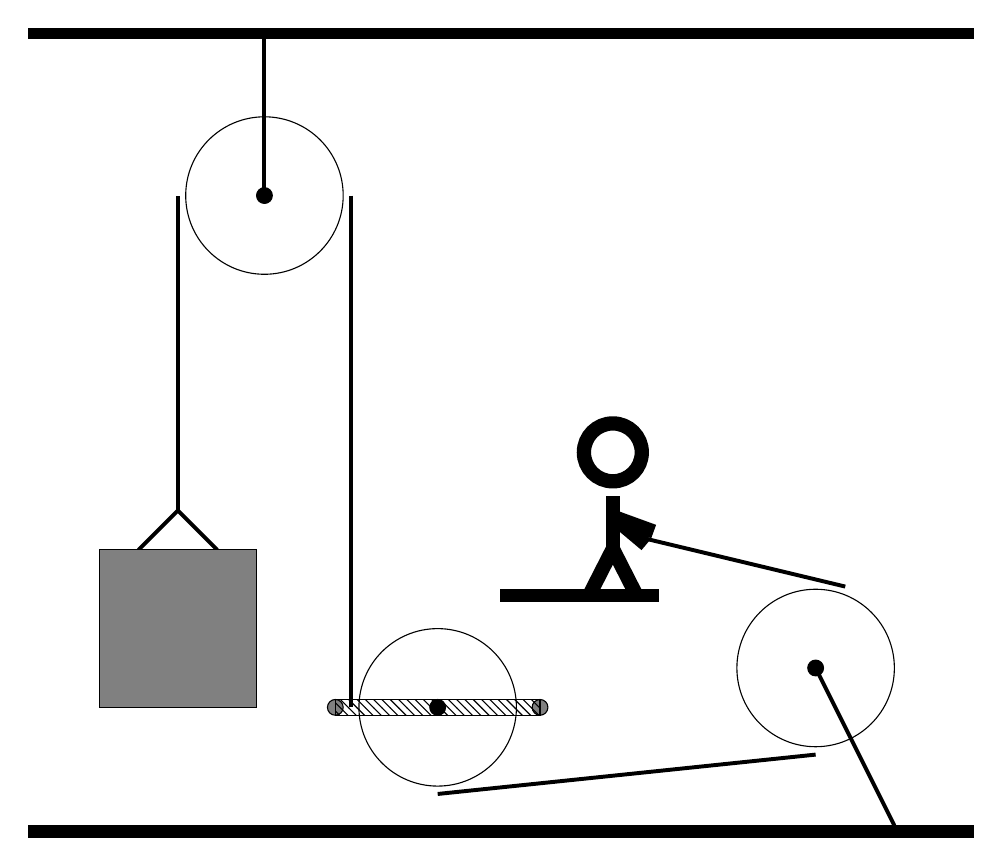
\begin{tikzpicture}
			 % Pulley diagrams will always start with the representation of a ceiling, formed using a rectangle like in the next line
			\draw[fill=black] (-2, 10) rectangle (10, 10.125);

			% The folloing l3 lines define a pulley. The large cicle (radius = 1) is the pulley wheel, which turns around the small circle (radius = 0.1). The 
			% third lline defines a supporting rope which connects the pulley to the ceiling.			
			\draw (1, 8) circle (1);
			\draw[fill=black] (1, 8) circle (0.1);
			\draw[line width=0.5mm] (1, 10) -- (1, 8);
			
			% This is also a  pulley. The first two lines are the pulley wheel and pivot point , as above. However, this pulley  attached to a backing well 
			% rather than hung from the ceiling. The support structures are defined by two small supporrting  pins (the 3rd and 4th lines below this one
			% and the rectangle with north west line patterning.
			\draw[fill=white](3.2, 1.5) circle (1);
			\draw[fill=black] (3.2, 1.5) circle (0.1);
			\draw[fill=black!50] (4.5, 1.5) circle (0.1);
			\draw[fill=black!50] (1.9, 1.5) circle (0.1);
			\draw[pattern=north west lines, pattern color=black] (1.9, 1.6) rectangle (4.5, 1.4);
			
			% This is another pulley, similar to the first, but this time the supporting rope is affixed to the ground/floor
			\draw (8, 2) circle (1);
			\draw[fill=black] (8, 2) circle (0.1);
			\draw[line width=0.5mm] (8, 2) -- (9, 0);
			
			% Th is is the weight, usually depicted using a 2x2 rectangle and two line segments aranged in a triangle shape and meant to depict guy wires by which the
			%  weight is hung from the rope running through the pulley system
			\draw[line width=0.5mm](-0.6, 3.5) --  (-0.1, 4.0) -- (0.4, 3.5);
			\draw[fill=black!50] (-1.1, 3.5) rectangle (0.9, 1.5);
			
			% This is the rope. This will mostly start from the weight and run sequentially through the system to the fugure pulling the rope. 
			% The rope will be depicted using a combination of lines (straight segments between pulleys) and calls to the \centrearc function, where the rope
			% runs over pulleys
			% The rope starts at the weight and runs up to the first pulley located at (1, 8) 
			\draw[line width=0.5mm] (-0.1, 4.0) -- (-0.1, 8);
			% The rope runs  180 deg. over the first pulley located at (1, 8) 
			\centerarc[line width=0.5mm](1, 8)(180:0:1.1)
			% The rope runs down from the first pulley to the second pulley, the one affixed to the walls located at (3.2, 1.5)
			\draw[line width=0.5mm](2.1, 8) -- (2.1, 1.5);
			% The rope runs 90 deg around the second pulley,
			\centerarc[line width=0.5mm](3.2, 1.5)(180:270:1.1);
			% From there the rope runs horizontally over to the last pulley located at (8, 2)
			\draw[line width=0.5mm](3.2, 0.4) -- (8, 0.9);
			% The rope runs 160 degrees   around the last pulley
			\centerarc[line width=0.5mm](8, 2)(270:430:1.1);
			 % Finally, the rope runs from the last pulley to the figure pulling  
			\draw[line width=0.5mm](8.376, 3.034) -- (5.6, 3.7);
			
			% This represents a figure (a stick figure, drawn using \Strichmaxerl) who is meant to be pulling on the loose end of the 
			% rope running through the pulley system. In this case, the figure is standing on an elevated platform represented by the rectangle two lines below this.		
			\node at (5.5, 4) {\Strichmaxerl[10][140][-20]};
			\draw[fill=black] (4, 3) rectangle (6, 2.85);
			
			% The last element of these pulley designs is always a rectangle repicting a "floor"
			\draw[fill=black] (-2, 0) rectangle (10, -0.15);
	\end{tikzpicture}
\end{document}